\section{Introduction}
\label{sec:introduction}

Large language models answer factual questions from knowledge stored in their
weights, and that knowledge is incomplete, frozen at training time, and
expensive to change. Retrieval-Augmented Generation
(RAG)~\cite{lewis2020rag} addresses all three problems at once: instead of
asking the model to remember, the system searches an external document
collection for passages relevant to the question and places them in the
model's context, so that the model reads rather than recalls. The technique
has become the default way of grounding language models in private,
fresh, or specialised document collections, and a large family of
architectural refinements has grown around it: lexical--dense hybrid
retrieval, cross-encoder reranking, hypothetical document embeddings,
corrective retrieval, iterative retrieval interleaved with reasoning, and
routers that pick a strategy per question.

The difficulty, for anyone who has to choose among these architectures, is
that each refinement is usually evaluated by its authors on their own stack
--- their own corpus, chunking, retriever, generator, and prompts --- and
against a small set of baselines. Published numbers are therefore rarely
comparable across papers, and improvements measured on one stack routinely
fail to transfer to another. Worse, our measurements show that the
refinements are not uniformly safe: the strongest single retrieval
improvement we measure, cross-encoder reranking, gains
$+0.051$ Exact Match over the standard baseline on HotpotQA and
\emph{loses} $-0.100$ on NaturalQuestions --- a catastrophic regression that
a single-benchmark evaluation would never reveal. Practitioners deploying
RAG face a menu of architectures whose relative merits depend on the
question distribution in ways the literature does not document.

This article makes three contributions.

\begin{enumerate}
\item \textbf{A controlled, statistically grounded comparison of thirteen
RAG architectures.} Every architecture is evaluated on the same 21-million-passage
Wikipedia corpus, the same embedding model, the same vector database, the
same generator, and the same answer prompt, over five question sets
(NaturalQuestions, TriviaQA, HotpotQA, 2WikiMultihopQA, MuSiQue) totalling
more than 37{,}000 questions --- so that the only difference between two rows of
a results table is the architecture itself. Differences are tested with
paired statistics (McNemar's test on Exact Match, Wilcoxon signed-rank on
continuous metrics) under a Holm correction, and every retrieval figure is
reported against the ceiling the corpus imposes, which we measure. Budget-matched
controls separate ``a better architecture'' from ``more text in the
context'', and abstention is measured separately from error, which reverses
one published-style conclusion (Section~\ref{sec:results}).

\item \textbf{A diagnosis of \emph{why} retrieval fails.} Aggregate recall
cannot distinguish failure causes that call for entirely different fixes. We
classify the baseline's retrieval failures into five causes --- wrong slice
of the right article, right article ranked too low, article unreachable by
the question's own vocabulary, no gold article stating the answer, and
article absent from the corpus --- and show that the distribution of causes,
not any aggregate score, predicts which architectural refinement pays off
on which question set.

\item \textbf{CascadeRAG, a cascade architecture built from the
diagnosis.} CascadeRAG combines a fused first stage --- dense, lexical, and cross-encoder rankings
merged by Reciprocal Rank Fusion, which avoids the reranker's collapse
while keeping most of its gain --- with \emph{abstention-triggered
escalation}: only when the reader itself declines to answer, having seen
the retrieved passages, is the question handed to a more expensive
strategy. The trigger is a \emph{posterior} signal, unlike routers that
predict difficulty from the question alone, and it is \emph{lossless} under
Exact Match: across all 887{,}917 (question, architecture) pairs measured
here, no abstention ever scores Exact Match~1, so escalation cannot discard
a correct answer. Against every baseline on every question set CascadeRAG
wins \ResultWins{} of \ResultPairs{} paired comparisons, loses
\ResultLosses{}, and ties \ResultTies{}, at 1.16--1.58 generator calls per
question --- against 2.3 for iterative retrieval and 3.0 for corrective
RAG. The result replicates under a second, unrelated generator.
\end{enumerate}

\begin{figure}[t]
\centering
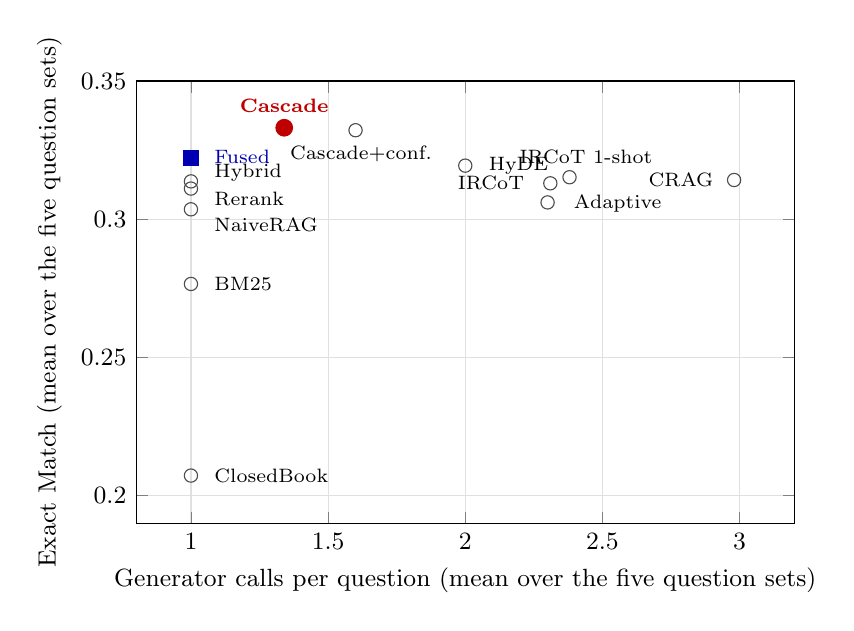
\begin{tikzpicture}
\begin{axis}[
    width=0.82\textwidth, height=7.2cm,
    xlabel={Generator calls per question (mean over the five question sets)},
    ylabel={Exact Match (mean over the five question sets)},
    xmin=0.8, xmax=3.2, ymin=0.19, ymax=0.35,
    grid=major, grid style={black!12},
    tick label style={font=\small}, label style={font=\small},
    every node near coord/.append style={font=\scriptsize}
]
% Means computed from the per-set generated fragments (paper/*.gen.tex);
% per-set values and significance tests are in Section 7.
\addplot[only marks, mark=o, mark size=2.4pt, black!70] coordinates {
    (1.00,0.2073) (1.00,0.2766) (1.00,0.3036) (1.00,0.3137) (1.00,0.3111)
    (2.00,0.3194) (2.98,0.3142) (2.31,0.3130) (2.38,0.3152) (2.30,0.3061)
    (1.60,0.3322)
};
\addplot[only marks, mark=square*, mark size=2.6pt, blue!70!black] coordinates {
    (1.00,0.3222)
};
\addplot[only marks, mark=*, mark size=3pt, red!75!black] coordinates {
    (1.34,0.3331)
};
\node[font=\scriptsize, anchor=west] at (axis cs:1.05,0.2073) {ClosedBook};
\node[font=\scriptsize, anchor=west] at (axis cs:1.05,0.2766) {BM25};
\node[font=\scriptsize, anchor=west] at (axis cs:1.05,0.2980) {NaiveRAG};
\node[font=\scriptsize, anchor=west] at (axis cs:1.05,0.3170) {Hybrid};
\node[font=\scriptsize, anchor=west] at (axis cs:1.05,0.3075) {Rerank};
\node[font=\scriptsize, anchor=west, blue!70!black] at (axis cs:1.05,0.3225) {Fused};
\node[font=\scriptsize, anchor=west] at (axis cs:2.05,0.3194) {HyDE};
\node[font=\scriptsize, anchor=east] at (axis cs:2.94,0.3142) {CRAG};
\node[font=\scriptsize, anchor=east] at (axis cs:2.25,0.3130) {IRCoT};
\node[font=\scriptsize, anchor=south] at (axis cs:2.44,0.3165) {IRCoT 1-shot};
\node[font=\scriptsize, anchor=west] at (axis cs:2.36,0.3055) {Adaptive};
\node[font=\scriptsize, anchor=south, red!75!black] at (axis cs:1.34,0.3350) {\textbf{Cascade}};
\node[font=\scriptsize, anchor=north] at (axis cs:1.62,0.3300) {Cascade+conf.};
\end{axis}
\end{tikzpicture}
\caption{Answer quality against generator cost for every architecture
measured in this article, averaged over the five question sets. The
proposed cascade (red) reaches the highest mean Exact Match at a fraction
of the cost of the iterative and corrective methods; its first stage alone
(Fused, blue) already dominates the single-call architectures. Per-set results,
in which no single architecture wins everywhere, are analysed in
Section~\ref{sec:results}.}
\label{fig:pareto}
\end{figure}

A fourth, methodological contribution runs through the article: every
number reported here --- every cell of every table, including those in this
sentence --- is generated by the benchmark code directly from the
per-question output files and imported into the manuscript as a named
macro, so no figure can drift from the experiment that produced it. The
benchmark, the analysis tools, and the manuscript build are one
reproducible pipeline.

The article is organised for two audiences. Sections~\ref{sec:background}
and~\ref{sec:architectures} are self-contained: they explain how RAG works
--- embeddings, similarity search, vector databases, and why retrieval is
preferred to retraining --- and then describe each compared architecture
with a uniform template and diagram, so that a reader new to the area can
follow the rest. Sections~\ref{sec:cascade}--\ref{sec:results} present the
proposed architecture, the experimental protocol, and the results;
Section~\ref{sec:discussion} distils practical guidance;
Section~\ref{sec:limitations} states limitations.
